\chapter[LaTeX]{Ukážky užitočných príkazov v systéme LaTeX}
\label{kap:latex}

V tejto kapitole si ukážeme príklady niektorých užitočných príkazov,
ako napríklad správne používanie tabuliek a obrázkov, číslovanie
matematických výrazov a podobne. Konkrétne príkazy použité v tejto
kapitole nájdete v zdrojovom súbore \verb'latex.tex'.  Všimnite si, že
pre potreby obsahu a hlavičky stránky je v zdrojovom súbore uvedený aj
skrátený názov tejto kapitoly. Ďalšie užitočné príkazy nájdete aj v
kapitole \ref{kap:clenenie}, na ktorú sme sa na tomto mieste odvolali
príkazom \verb'\ref'.

\section{Obrázky}

Vašu prácu ilustrujte vhodnými obrázkami. Pri použití programu
pdflatex je potrebné pripraviť obrázky vo formáte pdf, jpg alebo
png. Vektorové obrázky (napr. eps, svg) je najvhodnejšie skonvertovať
do formátu pdf, napríklad programom Inkscape.

Na vkladanie obrázkov použite prostredie \verb'figure', ktoré obrázok
umiestni na vhodné miesto, väčšinou na vrch alebo spodok stránky a
tiež sa stará o automatické číslovanie obrázkov. Na každý obrázok sa
treba v hlavnom texte odvolať. Napríklad ilustráciu hry Červík vidíme
na obrázku \ref{obr:cursus}. Pri odvolávaní sa na číslo obrázku
používame príkaz \verb'\ref'. Pri vložení alebo zmazaní obrázku tak
nemusíme ručne všetky ostatné obrázky prečíslovať.

\begin{figure}
%vlozenie samotneho obrazku vycentrovaneho a vhodnej velkosti
%obrazok je v subore images/cervik.png
\centerline{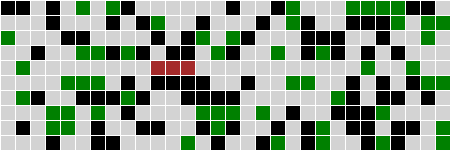
\includegraphics[width=0.4\textwidth]{images/cervik}}
%popis obrazku
\caption[Ukážka hry Červík]{Ukážka hry Červík. Červík je znázornený červenou farbou, voľné políčka sivou, jedlo zelenou a steny čiernou. Hoci tento popis obrázku je dlhší, v zdrojovom texte je aj kratšia verzia, ktorá sa zobrazí v zozname obrázkov.}
%id obrazku, pomocou ktoreho sa budeme na obrazok odvolavat
\label{obr:cursus}
\end{figure}

Podobne tabuľky vkladajte pomocou prostredia \verb'table', pričom
samotnú tabuľku vytvoríte príkazom \verb'tabular'. Každú tabuľku potom
spomeňte aj v hlavnom texte. Napríklad v tabuľke \ref{tab:cas}
vidíme porovnanie časov niekoľkých fiktívnych programov.

\begin{table}
% v tabulke sa popis zvykne davat nad tabulku
\caption[Doba výpočtu a operačná pamäť potrebná na spracovanie vstupu XYZ]{Doba výpočtu a operačná pamäť potrebná na spracovanie vstupu XYZ. V tomto popise môžeme vysvetliť detaily potrebné pre pochopenie údajov v tabuľke.}
%id tabulky
\label{tab:cas}
% tu zacina samotna tabulka
\begin{center}
\begin{tabular}{lrr}
\hline 
Meno programu & Čas (s) & Pamäť (MB) \\
\hline
Môj super program & 25.6 & 120 \\
Speedy 3.1  & 32.1 & 100 \\
VeryOld & 244.1 & 200 \\
\hline
\end{tabular}
\end{center}
\end{table}

V texte môžete tiež potrebovať dlhšie matematické výrazy, ako napríklad tento
\begin{equation}
\sum_{k=0}^n q^k = \frac{q^{n+1}-1}{q-1}.
\label{eq:geom}
\end{equation}
Použitím prostredia \verb'equation' bol tento výraz zarovnaný na stred na
zvláštnom riadku a očíslovaný. Na toto číslo sa tiež môžeme odvolať
príkazom \verb'\ref'. Napríklad rovnica (\ref{eq:geom}) predstavuje súčet 
geometrickej postupnosti.

Napokon, v texte nezabudnite citovať použitú literatúru pomocou
príkazu \verb'\cite' Napríklad ďalšie detaily o systéme LaTeX nájdete
v knihe od Tobiasa Oetikera a kolektívu \cite{Oetiker2000}. Pre ukážku
citujeme aj článok z vedeckého časopisu \cite{clanok} a článok z
konferencie \cite{clanok_na_konferencii}, technickú správu
\cite{technical_report}, knihu \cite{kniha} a materiál z internetu
\cite{smernica}.


